\section{Another Method: Computational Graphs}
In the optimal control section, in essence, we try to minimize the cost of many many variables, this is a similar problem that to teaching neural networks and machine learning, we might be able to borrow some tricks and method they use to solve our problem.

Instead of thinking of a cost function as just a function, we can treat it as a \textit{computational graph}. We'll discuss briefly about what's a computational graph and how can we implement GRAPE using one. We won't go in depth as we did in the chapter on optimal control, it's only a general overview meant to show an alternative method. Let's start by defining a computational graph\footnote{Of course, graph theory is an entire field of mathematics by itself and we can't really give a rigorous definition, but more of an intuitive explanation}.

\subsection{What are Computational Graphs}
A computational graph consists of nodes and connection between them, a node can be one of one of three things
\begin{itemize}
    \item \textbf{Operations}, the operation takes a list of numbers from other nodes and outputs another list of numbers (doesn't need to be of same size) % TODO: Change wording of this line
    \item \textbf{Parameters}, these are, as the name suggests, the parameters of the graph and can be used by the operations.
    \item \textbf{Variables}, these are the variables that of the graph, and they too can be used by the operators of the graph
\end{itemize}
The graph starts as the variables, goes through some operations that use parameters and gives out some resualt. Let's take a look at a simple example

\begin{figure}[H]
    \centering
    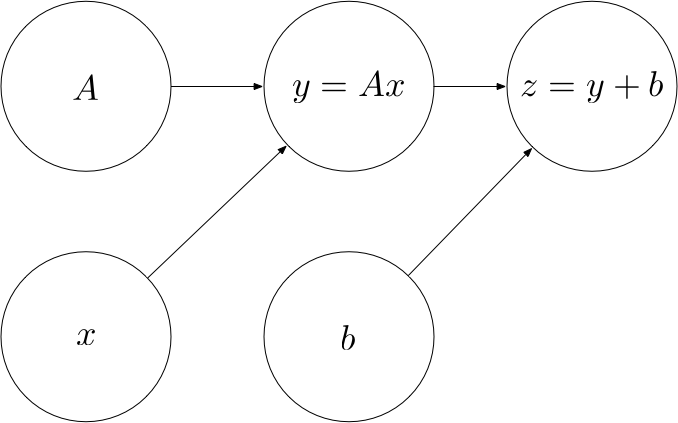
\includegraphics[width=0.4\columnwidth]{Example-comp-graph.png}
    \caption{Example of a basic computational graph}
    \label{fig:example-computational-graph}
\end{figure}

Here, $x$ is the variable, $A$ and $b$ are the parameters, and $y$ and $z$ are the operators. The function that this graph represents is $y = a \cdot e^{x}$. For now it properly seems overkill to use the graph to represent that simple of a function but in the next two sections you'll see the magic of the computational graph, in terms of thinking about the gradient.

\subsection{Back-Propagation}
This is the magic of the computational graph, calculating the gradient of the cost function by back-propagating the derivatives to the initial variables. The idea is simple, instead of trying to directly calculating the gradient, we calculate the derivative of node by the previous node, and relate the cost function to the variables by the chain rule. What does that mean, let's show an example.

Let's say we have a simple computational graph that looks like
\[x \rightarrow L_1 \rightarrow L_2 \rightarrow L_3 \rightarrow y\] 
and we want to calculate the derivative, $\frac{\partial y}{\partial x}$. Instead of calculating the derivative directly, we can back-propagate the derivative as
\[\frac{\partial y}{\partial x} = \frac{\partial y}{\partial L_3} \cdot \frac{\partial L_3}{\partial L_2} \cdot \frac{\partial L_2}{\partial L_1} \cdot \frac{\partial L_1}{\partial x} \cdot \frac{\partial y}{\partial x}\]
luckily for us each operation is very simple so each derivative is simple as well.

\subsection{GRAPE in a Computational Graph}
Now we can finally implement grape as a computational graph, we'll consider the simplest case of GRAPE, no constraints, only the original definition (see equations \ref{eq:fidelity_sim}, \ref{eq:U_def_prod} and \ref{eq:hamiltonianl_form})%\footnote{This is assuming only one drive hamiltonian, for more drives the only difference is adding $\epsilon'_k H'_d$ and so on for each drive} %TODO: Change wording of footnote and add explenation where the function comes from
\[
    F (\vec{\epsilon}) = \abs{\bra{\psi_{target}} \prod_{i=0}^N e^{-i \cdot \delta t  (H_0 + \epsilon_k H_d)} \ket{\psi_{initial}}}^2
\]
In this case, $\vec{\epsilon}$ is the variable, $H_0$, $-i \cdot \delta t$, $\bra{\psi_{target}}$ and $\ket{\psi_{initial}}$ are the parameters. They relate through the operators and everything can be displayed as the following graph\footnote{Simplifying for 3 time steps, to add more time steps is pretty straight forward}

\begin{center}
\begin{tikzpicture}[scale=2.3]
\renewcommand*{\VertexLineWidth}{1pt}%vertex thickness
\renewcommand*{\EdgeLineWidth}{1pt}% edge thickness
\GraphInit[vstyle=Normal]
% Variables
\Vertex[L={\Huge $\epsilon_0$}, x=0,y=5]{e0}
\Vertex[L={\Huge $\epsilon_1$},x=1,y=5]{e1}
\Vertex[L={\Huge $\epsilon_2$},x=2,y=5]{e2}

\Vertex[L=$-i \delta t H_d$,x=-0.5,y=4.5]{idt00}
\Vertex[L=$-i \delta t H_d$,x=0.5,y=4.5]{idt01}
\Vertex[L=$-i \delta t H_d$,x=1.5,y=4.5]{idt02}
% L1
\Vertex[L=$\cdot$,x=0,y=4]{L10}
\Vertex[L=$\cdot$,x=1,y=4]{L11}
\Vertex[L=$\cdot$,x=2,y=4]{L12}

\Vertex[L=$-i \delta t H_0$,x=-0.5,y=3.5]{idt10}
\Vertex[L=$-i \delta t H_0$,x=0.5,y=3.5]{idt11}
\Vertex[L=$-i \delta t H_0$,x=1.5,y=3.5]{idt12}
% L2
\Vertex[L=$+$,x=0,y=3]{L20}
\Vertex[L=$+$,x=1,y=3]{L21}
\Vertex[L=$+$,x=2,y=3]{L22}
% L3
\Vertex[L=$\exp$,x=0,y=2]{L30}
\Vertex[L=$\exp$,x=1,y=2]{L31}
\Vertex[L=$\exp$,x=2,y=2]{L32}
% L4
\Vertex[L=$\cdot$,x=1,y=1]{L4}

\Vertex[L=$\ket{\psi_{init}}$,x=2,y=0.7]{psii}
\Vertex[L=$\bra{\psi_{targ}}$,x=0,y=0.7]{psit}
% C
\Vertex[L=$\cdot$,x=1,y=0]{C}

%%%%%%%%%%%%%%%%%%%%%%%%%%%%%%
\draw [->]  (e0) edge  (L10);
\draw [->]  (e1) edge  (L11);
\draw [->]  (e2) edge  (L12);
\draw [->]  (idt00) edge  (L10);
\draw [->]  (idt01) edge  (L11);
\draw [->]  (idt02) edge  (L12);

\draw [->]  (L10) edge  (L20);
\draw [->]  (L11) edge  (L21);
\draw [->]  (L12) edge  (L22);
\draw [->]  (idt10) edge  (L20);
\draw [->]  (idt11) edge  (L21);
\draw [->]  (idt12) edge  (L22);

\draw [->]  (L20) edge  (L30);
\draw [->]  (L21) edge  (L31);
\draw [->]  (L22) edge  (L32);

\draw [->]  (L30) edge  (L4);
\draw [->]  (L31) edge  (L4);
\draw [->]  (L32) edge  (L4);

\draw [->]  (L4) edge  (C);
\draw [->]  (psii) edge  (C);
\draw [->]  (psit) edge  (C);

\end{tikzpicture}
\end{center}
The layers are as follows

\begin{align*}
    L_1^k &= -i \delta t H_d \epsilon_k \\
    L_2^k &= -i\delta t H_0 + L_1^k \\
    L_3^k &= e^{L_2^k} \\
    L_4 &= \prod_{k=0}^N L_3^k \\
    C &= \bra{\psi_{target}} L_4 \ket{\psi_{initial}}
\end{align*}

And the derivatives are calculated rather easily as

\begin{align*}
    \frac{\partial L_1^k}{\partial \epsilon_k} &= -i \delta t H_d\\
    \frac{\partial L_2^k}{\partial L_1^k} &= 1 \\
    \frac{\partial L_3^k}{\partial L_2^k} &= e^{L_2^k} \\
    \frac{\partial L_4}{\partial L_3^k} &= \prod_{i \ne k} L_3^i \\
    \downarrow \\
    \frac{\partial C}{\partial \epsilon_k} &= \bra{\psi_{target}}  \frac{\partial L_4}{\partial L_3^k}  \frac{\partial L_3^k}{\partial L_2^k} \frac{\partial L_2^k}{\partial L_1^k}  \frac{\partial L_1^k}{\partial \epsilon_k} \ket{\psi_{init}}
\end{align*}
It's important to note that $\frac{\partial L_1^i}{\partial \epsilon_j} = 0$ for $i \ne j$ so we didn't refer to those derivative (This is true for the derivative between any two layers).

We now everything we need to implement GRAPE as a computational graph, and we can use a library, such as google's tensorflow, to find the optimal pulse.